\documentclass[a4paper, 11pt]{article}
\usepackage[top=2cm, bottom=2cm, left = 2cm, right = 2cm]{geometry} 
\geometry{a4paper} 

\usepackage[T1]{fontenc}
\usepackage[utf8]{inputenc}
\usepackage{lmodern}
\usepackage[ngerman]{babel}
\usepackage{microtype}


\usepackage{graphicx} 
\usepackage{amsmath,amssymb}  
\usepackage{bm}  
\usepackage[pdftex,bookmarks,hidelinks,breaklinks]{hyperref}  

\title{Praktikumsbericht Audiosignalverarbeitung}
\author{Franko Jolic, Janne Buhr}
%\date{}

\begin{document}
\AddToHook{cmd/section/before}{\clearpage}
\begin{titlepage}
    \maketitle
    \tableofcontents
    \vfill
\end{titlepage}

\section{Aufgabenblatt 1}

    \subsection{Frage 1}
    Wie funktioniert eine Authentifizierung mit SHH-Schlüsseldateien (SSH keys)? Was ist die Grundidee und wie welche Schritte müssen ausgeführt werden?
    \begin{itemize}
    \item -- 
    \end{itemize}
    
    \subsection{Frage 2}
    Wofür genau benötigt man eine virtuelle Umgebung? Was sind die Vorteile?
    \begin{itemize}
    \item -- 
    \end{itemize}
        

\section{Aufgabenblatt 2}

    \subsection{Kurzvortrag}
    Wird in der Datei vortrag.text weiter ausgeführt

\section{Aufgabenblatt 3}

    
    
    \begin{figure}
    \includegraphics[width =0.5\textwidth]{plot.png}
    \caption{Hier kommt die Bildunterschrift hin.}
    \label{fig : label1}
    % Abbildung kann im Text mit \ ref { fig : label1 }
    % referenziert werden
    \end{figure}


    \subsection{Was ist eine Frequenz?}
    
    \subsubsection{Frage 1}
    Bei akustischen Signalen entscheidet vorallem die Frequenz der Schwingungen über die wahrgenommene Tonhöhe. 
    Welche Frequenzen liegen im hörbaren Bereich\\
    Je nach Alter und individuellen Eigenschaften hören Menschen Frequenzen von 20 bis 20000 Hz.


    Länge voller wiederholung 1 drittel sekunde 

    \subsection{Das Abtasttheorem}
    Notiert eure Vermutungen zu den obigen Fragen an dieser Stelle!
    \subsubsection{Fragen und Antworten zur ersten Teilaufgabe}
    Welche Grundfrequenz hat das periodische Signal? 
    \begin{itemize}
    \item Das periodische Signal hat eine Grundfrequenz von 1Hz.  
    \end{itemize}
    Was sind die Frequenzen der sinus und kosinusförmigen Teilsignale?
    \begin{itemize}
        \item Die Frequenz des sinusförmigen Teils liegt bei 2Hz
        \item Die Frequenz des cosinusförmigen Teils setzt sich zusammen aus 1Hz + 3Hz also 4Hz 
    \end{itemize}
    Ließe sich das kontinuierliche Signal s\textsubscript{a}(t) nur aus den Abtastwerten rekonstruieren? Oder sind informationen verloren gegangen, die dies unmöglich machen?
    \begin{itemize}
        \item Durch die Verringerung der Abtastrate sind wichtige Informationen verloren gegangen, wie beispielsweise der weitere Verlauf der Funktion, sowie Minima und Maxima die nicht mehr deutlich sind 
        also kann man das kontinuierliche signal nicht mehr rekonstruieren.
    \end{itemize}
    Ändert die Abtastrate und schaut euch die entsprechenden Plots an. Welche Rolle könnte die Abtastrate dabei spielen?
    \begin{figure}
        \centering
        \includegraphics[width =0.5\textwidth]{Abild220.png}
        \caption{Abtastrate von 5}
        \label{fig : label2}
        % Abbildung kann im Text mit \ ref { fig : label1 }
        % referenziert werden
        \end{figure}
    
        \begin{figure}
            \centering
            \includegraphics[width =0.5\textwidth]{Abild221.png}
            \caption{Abtastrate von 10}
            \label{fig : label3}
            % Abbildung kann im Text mit \ ref { fig : label1 }
            % referenziert werden
            \end{figure}

            \begin{figure}
                \centering
                \includegraphics[width =0.5\textwidth]{Abild222.png}
                \caption{Abtastrate von 20}
                \label{fig : label4}
                % Abbildung kann im Text mit \ ref { fig : label1 }
                % referenziert werden
                \end{figure}
    
    
                    \begin{itemize}
                    \item Wie man unten anhand der 3 Abbildungen sieht haben wir die Abtastrate zuerst auf 5 runtergesetzt und danach auf 20 erhöht. 
                    Man erkennt ganz genau das wir desto höher unsere Abtastrate ist, unsere Abbildung immer näher an das Original rankommt.
                    \end{itemize}
    
    
   
    
    \subsubsection{Fragen und Antworten zur zweiten Teilaufgabe}

     Lässt sich das Originalsignal aus den Abtastwerten rekonstruieren?\\
     \begin{figure}[h]
        \centering
        \includegraphics[height=5cm, width = 7cm]{ABild231.png}
        \caption{Das rekonstruierte Bild anhand der Abtastwerte}
      \end{figure}
     \begin{itemize}
        \item Das Original wird nicht hundertprozentig rekonstruiert, jedoch ist es sehr Nahe am Original dran. Wie man in Abbildung 5 erkennt, fehlen uns nur die Ränder welche durch unser begrenztes Intervall nicht perfekt rekonstruiert werden.
        
    \end{itemize}
     Ist die Rekonstruktion für alle Funktionswerte gleich gut?\\

     \begin{figure}[h]
        \centering
        \includegraphics[height=5cm, width = 7cm]{ABild230.png}
        \caption{Das rekonstruierte Bild mit einem Wert fs=5}
      \end{figure}
     \begin{itemize}
        \item Nein, die Rekonstruktion wird besser desto höher der Wert. Dies sieht man anhand der Abbildungen sehr gut, desto kleiner der Wert desto schlechter das Ergebnis.
     \end{itemize}
     Woran könnte es liegen, wenn ihr hier unterschiede feststellt?\\
     \begin{itemize}
        \item Durch einen kleineren Wert werden weniger Informationen übergeben. Dadurch werden bei verschiedenen Werten die Rekonstruktionen viel besser da der Algorithmus die Punkte besser rekonstruieren kann bei einem fs-Wert der hoch ist
     \end{itemize}
     Was passiert, wenn ihr die Abtastrate verringert oder erhöht?\\
     
     \begin{figure}[h]
        \centering
        \includegraphics[height=5cm, width = 7cm]{ABild232.png}
        \caption{Das rekonstruierte Bild mit einem Wert fs=20}
      \end{figure}
     
     \begin{itemize}
        \item In Abbildung 6 sieht man gut was passiert wenn man die Abtastrate verringert. Die Rekonstruktion wird ungenauer. 
        \item In Abbildung 7 zeigt sich wie eine höhere Abtastrate auf die Rekonstruktion auswirkt. Im Vergleich zu einem Wert von 5 oder 10 ist 20 noch um ein kleines Stück genauer.
     \end{itemize}
     Gibt es einen kritischen Wert bei dem eine sich etwas grundsätzlich verändert?\\
     
     \begin{figure}[h]
        \centering
        \includegraphics[height=5cm, width = 7cm]{ABild232.png}
        \caption{Das rekonstruierte Bild mit einem Wert fs=6}
      \end{figure}
     \begin{itemize}
        \item Vergleicht man die Rekonstruktion mit dem Wert fs=5 aus Abbildung 6 und fs=6 aus Abbildung 8, so erkennt man klar wie der Sprung von 5 auf 6 eine klare Verbesserung der Rekonstruktion ist.
     \end{itemize}
     Beantwortet diese Fragen in eurem Bericht mit Hilfe von passenden Abbildungen. Entsprechen die Ergebnisse euren Vermutungen?\\
     \begin{itemize}
        \item Die Vermutung, dass durch eine höhere Abtastrate die Rekonstruktion genauer wird wurde erfüllt. Jedoch ist es eine Überraschung, dass es einen kritischen Wert gibt und die Rekonstruktion bei einem Sprung von 5 auf 6 so drastisch anders ist.
     \end{itemize}

    \subsection{Frage 5}
    Wie verhalten sich die Frequenz des Signals und die Mindestabtastrate zu einander?
    Wie passt eure Beobachtung hier zu den Beobachtungen für das zusammengesetzte Signal s\textsubscript{a}?

    \subsection{Frage 6}
    Das berühmte und wichtige Abtasttheorem formalisiert eure Beobachtungen. Könnt ihr es formulieren?
    \begin{itemize}
    \item Das Abtasttheorem besagt, dass wir ein Signal rekonstruieren, sofern wir mindestens doppelt so viele Werte abgetastet haben wie unsere Frequenz.
    \end{itemize}
    
\section{Aufgabenblatt 4}

\subsection{Aliasing in Audio- und Bilddaten}

\subsubsection{Beispiel: Aliasing beim Abtasten eines Bildes}

Ab welchem Downsamplingfaktor könnt ihr eine Veränderung im Bild warhnehmen? Wie äußert sich das Aliasing im Bild?
    
\begin{figure}[h]
    \centering 
    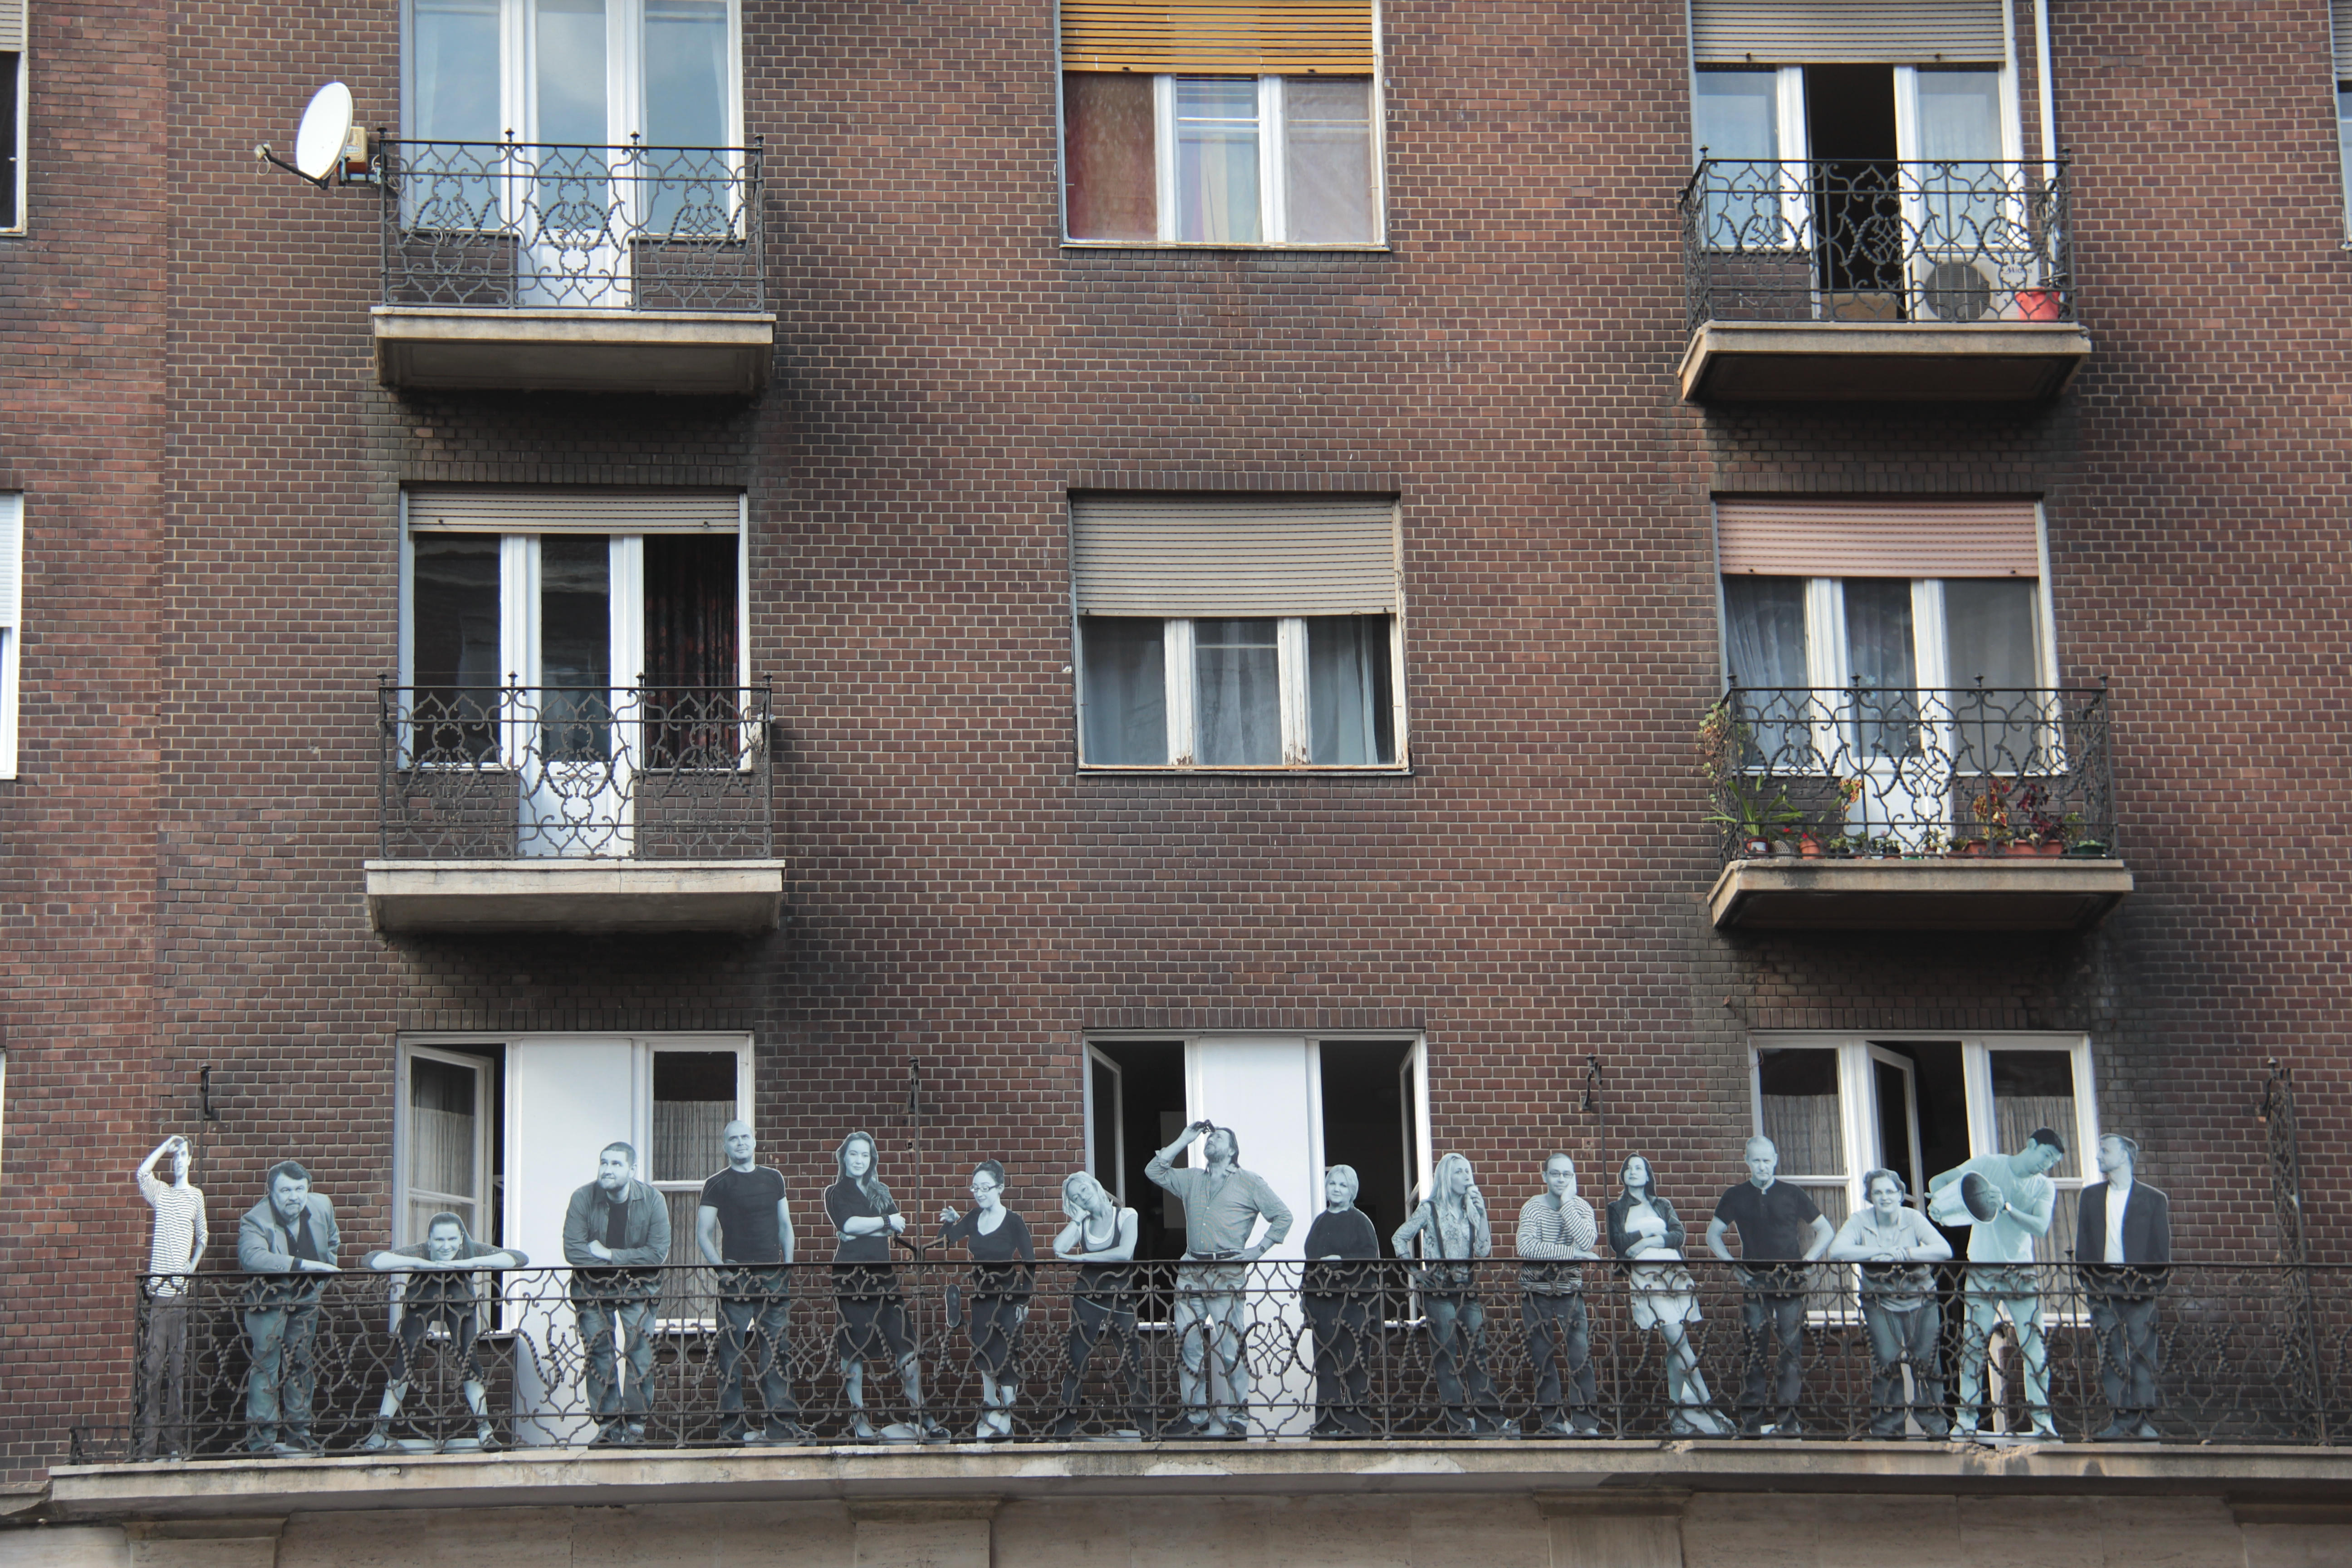
\includegraphics[width =0.5\textwidth]{test.png}
    \caption{Originalbild}
    \label{fig : label5}
\end{figure}
    
\begin{figure}[h]
    \centering 
    \includegraphics[width =0.5\textwidth]{test_sliced5.png}        \caption{Downsamplingfaktor 5}
    \label{fig : label6} 
\end{figure}
    
\begin{figure} [h]
    \centering 
    \includegraphics[height = 5cm , width =0.5 \textwidth]{test_sliced10.png}
    \caption{Downsamplingfaktor 10}
    \label{fig : label7}
\end{figure} 
     
    \begin{itemize}
    \item Oben sieht man unser Bild im Original und dann mit einem Downsamplingfaktor von 5 und 10. Wie man erkennt sind ab dem Downsamplingfaktor von 10 die Texturen ohne ranzuzoomen schon sehr ,,blurry''. Das Aliasing äußert sich im Bild daran, dass das Bild viel verschwommener aussieht.
    \end{itemize}
Fügt die beiden Bilder mit der geringern Auflösung nebeneinander in den Bericht ein. Sind im mit resize erzeugten Bild auch Aliasing-Effekte zu sehen? Wie unterscheidet sich dieses Bild vom Original? Warum sehen die beiden verkleinerten Bilder so unterschiedlich aus?
    \begin{itemize}
    \item -- 
    \end{itemize}
    
\subsubsection{Abtastung von Audiosignalen}

Könnt ihr Aliasing-Effekte ausmachen? Wie äußern sich diese?
    \begin{itemize}
    \item -- 
    \end{itemize}

\subsection{Quantisierung}

Wie viele Werte kann ein 16-bit Integer repräsentieren? Was ist der größte und was der kleinste darstellbare Wert?
    \begin{itemize}
    \item -- 
    \end{itemize}
Wie hängen Wortbreite n und die Anzahl der Quantisierungsschritte zusammen?
    \begin{itemize}
    \item -- 
    \end{itemize}
Ab welcher Wortbreite ist die Quantisierung deutlich sichtbar? Füge die Plots zur Illustration im Bericht hinzu.   
    \begin{itemize}
    \item --  
    \end{itemize}
Ab welcher Wortbreite kannst du das Quantisierungsrauschen im Signal hören?  
    \begin{itemize}
    \item --
    \end{itemize} 
Wiederhole die Experimente von oben mit den neuen Signalen und erläutere im Bericht anhand von entsprechenden Plots und Kenngrößen was man bei der Aufnahme von Audio beachten sollte um den Quantisierungsfehler möglichst klein zu halten.    
    \begin{itemize}
    \item --
    \end{itemize} 
\section{Aufgabenblatt 5}

\section{Aufgabenblatt 6}

\section{Aufgabenblatt 7}

\section{Aufgabenblatt 8}

\section{Aufgabenblatt 9}

\section{Aufgabenblatt 10}

\end{document}